% Использован шаблон:
% https://www.writelatex.com/coursera/latex/1.1
% http://coursera.org/course/latex


\documentclass[a4paper,12pt]{article}

\usepackage{cmap}
\usepackage[T2A]{fontenc}
\usepackage[utf8]{inputenc}
\usepackage[english,russian]{babel}
\usepackage{fancyhdr}
\usepackage{minted}
\usepackage{hyperref}
\usepackage{amsmath}
\usepackage{graphicx}

\hypersetup{
  pdfborderstyle={/S/U/W 1}
}

\graphicspath{{./images/}}

\pagestyle{fancy}
\fancyhf{}
\lhead{Антон Завьялов, ПИ-72}
\rhead{\textbf{Лабораторная №1. Вариант 7}}
\cfoot{\thepage}

\makeatletter
\def\@seccntformat#1{%
  \expandafter\ifx\csname c@#1\endcsname\c@section\else
  \csname the#1\endcsname\quad
  \fi}
\makeatother

\begin{document} % Конец преамбулы, начало текста.

\begin{center}
  \textbf{Лабораторная работа №1 по дисциплине\linebreak"Компьютерная графика"\linebreak\linebreakВыполнил студент группы ПИ-72 Завьялов А.А.}\\
\end{center}

\section{\normalsize{Задание}}
\begin{flushleft}
  Разработать программу аффинных преобразований и проецирования 3D-проволочного объекта. Интерфейс должен позволять управлять текущим преобразованием объекта мышью или клавиатурой.
\end{flushleft}

\begin{flushleft}
  Реализовать все элементарные преобразования. Кроме того, реализовать дополнительное динамическое преобразование (анимацию) по варианту.
  \linebreak\linebreak
  \textbf{Вариант 7.} Вращение относительно геометрического центра объекта со случайной сменой направления (смена направления должна осуществляться плавно!)
\end{flushleft}

\section{\normalsize{Ход работы}}
\begin{flushleft}
  \begin{enumerate}
    \item Реализован алгоритм Брезенхэма растеризации отрезка \(((x_0, y_0),(x_1,y_1))\).
    \item Написан простой парсер файлов в формате \href{https://ru.wikipedia.org/wiki/Obj}{Wavefront OBJ}. Модель парсится в список вершин \([v_0 = (x, y, z), v_1, v_2, ..., v_n]\) и список граней \([f_0 = (v_i, v_{i+1}, ..., v_k), ..., f_m]\).
    \item Реализованы 4 основных типа аффинных преобразований: перемещение, поворот (вокруг осей OX, OY, OZ), масштабирования, отражения (относительно плоскостей XY, XZ, YZ).
    \item Написана процедура перспективного проецирования с центром проецирования в точке \((c, 0, 0)\) и проекционной плоскостью ZOY. \linebreakМатрица преобразования: \(\begin{pmatrix}0 & 0 & 0 & - 1/c \\ 0 & 1 & 0 & 0 \\ 0 & 0 & 1 & 0 \\ 0 & 0 & 0 & 1\end{pmatrix}\).\linebreak После преобразования координаты делятся на w и тройка координат \((0, y, z)\) преобразуется в пару координат \((y, z)\) экранного пространства. 
    \item Написана процедура проецирования ребер трехмерной фигуры на экранную плоскость и растеризации полученных линий.
    \item Реализованы 2 режима работы программы:
      \linebreak
      \begin{itemize}
        \item Формирование матрицы преобразования путем ввода команд в терминале. Поддерживаемые команды:
          \linebreak
          \begin{itemize}
            \item \textbf{translate | t} ox oy oz - перенос на \((ox, oy, oz)\)
            \item \textbf{scale | s} sx sy sz - масштабирование с коэффициентами \((sx, sy, sz)\)
            \item \textbf{rotation | r} angle [x | y | z] - поворот на угол angle вокруг заданной оси
            \item \textbf{mirror | m} [xy | yz | xz] - отражение относительно заданной плоскости
            \item \textbf{reset} - восстановление исходной матрицы преобразования (единичной матрицы)
            \item \textbf{quit | q} - завершение работы программы
          \end{itemize}
          После ввода команды к текущей матрице преобразования слева применяется новое преобразование (т.е., получается суперпозиция преобразований). Происходит перерисовка содержимого экрана с учетом получившегося преобразования.
        \item Динамическое преобразование (анимация) по варианту. Вращение относительно геометрического центра объекта со случайной (плавной) сменой направления подкреплено математической моделью.\linebreak\linebreakСначала единожды вычисляется суперпозиция поворотов вокруг осей OZ, OY, OX на углы \(\gamma, \beta, \alpha\) (углы не зафиксированны, т.е. можно совершить подстановку и получить конкретную матрицу).\linebreak\linebreakВ начале отсчета углы нулевые. Во времени осуществляется приращение углов на величины \(\Delta\alpha, \Delta\beta, \Delta\gamma\), эти приращения являются скоростями, которые изменяются на некоторые ускорения. Ускорения - постоянные величины, которые через некоторый промежуток времени t меняются случайным образом на некотором диапазоне.\linebreak\linebreakДалее углы подставляются в матрицу, получившееся преобразование трансформирует координаты точек модели.
      \end{itemize}
  \end{enumerate}
\end{flushleft}

\section{\normalsize{Исходный код}}
Исходный код программы также расположен в Git-репозитории по адресу: \url{https://github.com/andiogenes/cg/tree/master/wireframe}
\inputminted[breaklines]{python}{../wireframe.py}

\section{\normalsize{Демонстрация работы программы}}
\begin{flushleft}
  Перемещение:
  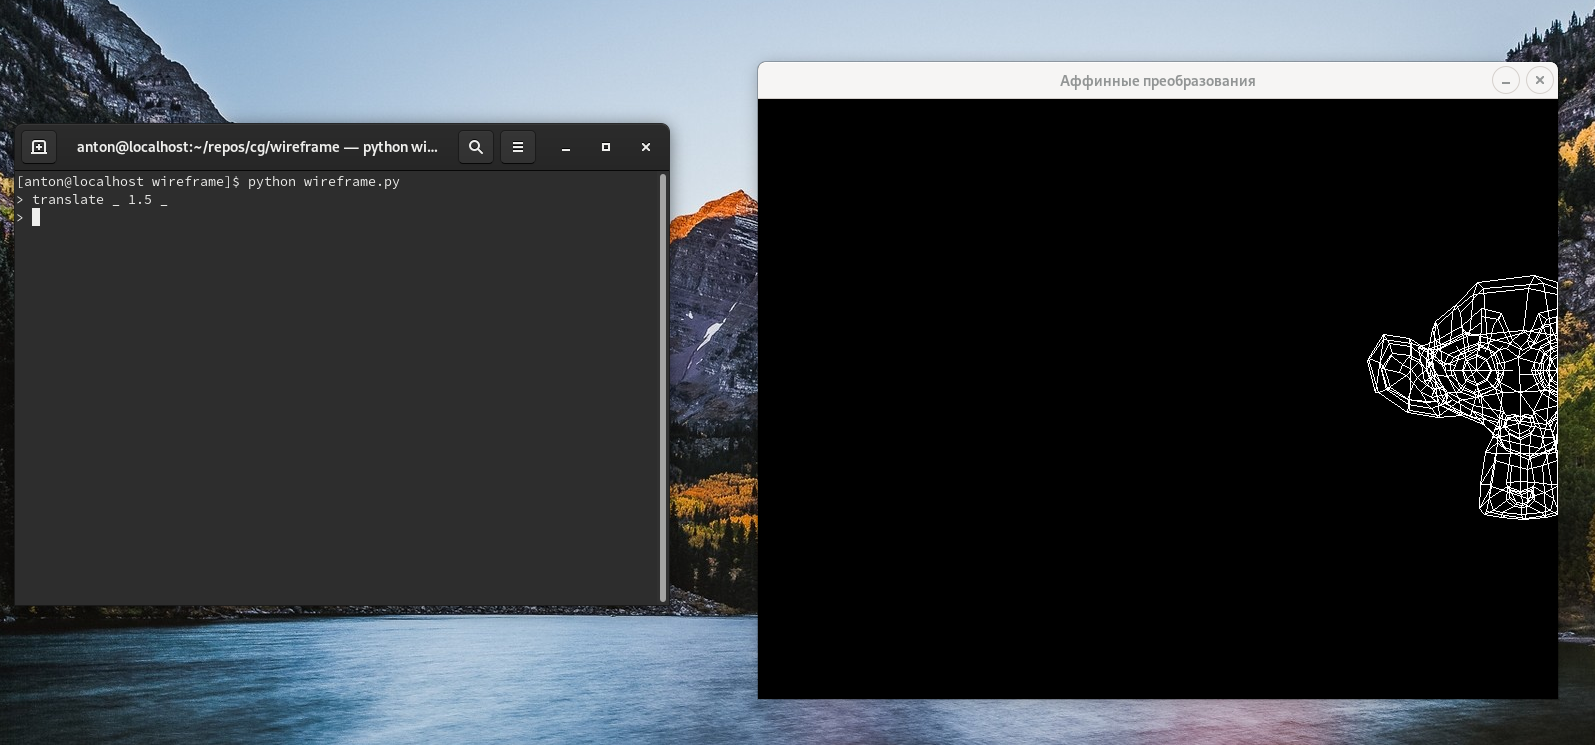
\includegraphics{translation.png}
  Перспективная проекция (модель переместили ближе к камере):
  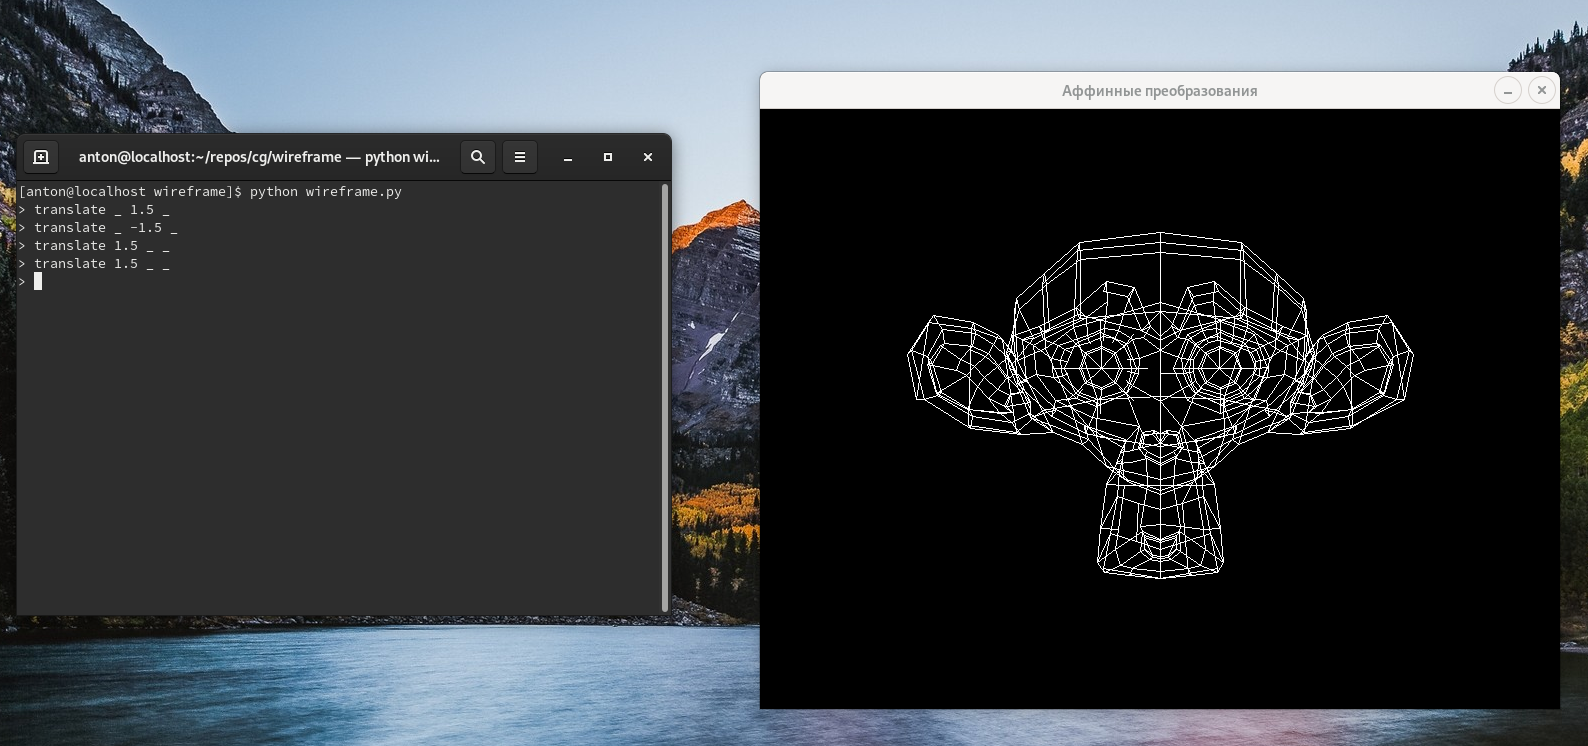
\includegraphics{perspective.png}
  Поворот:
  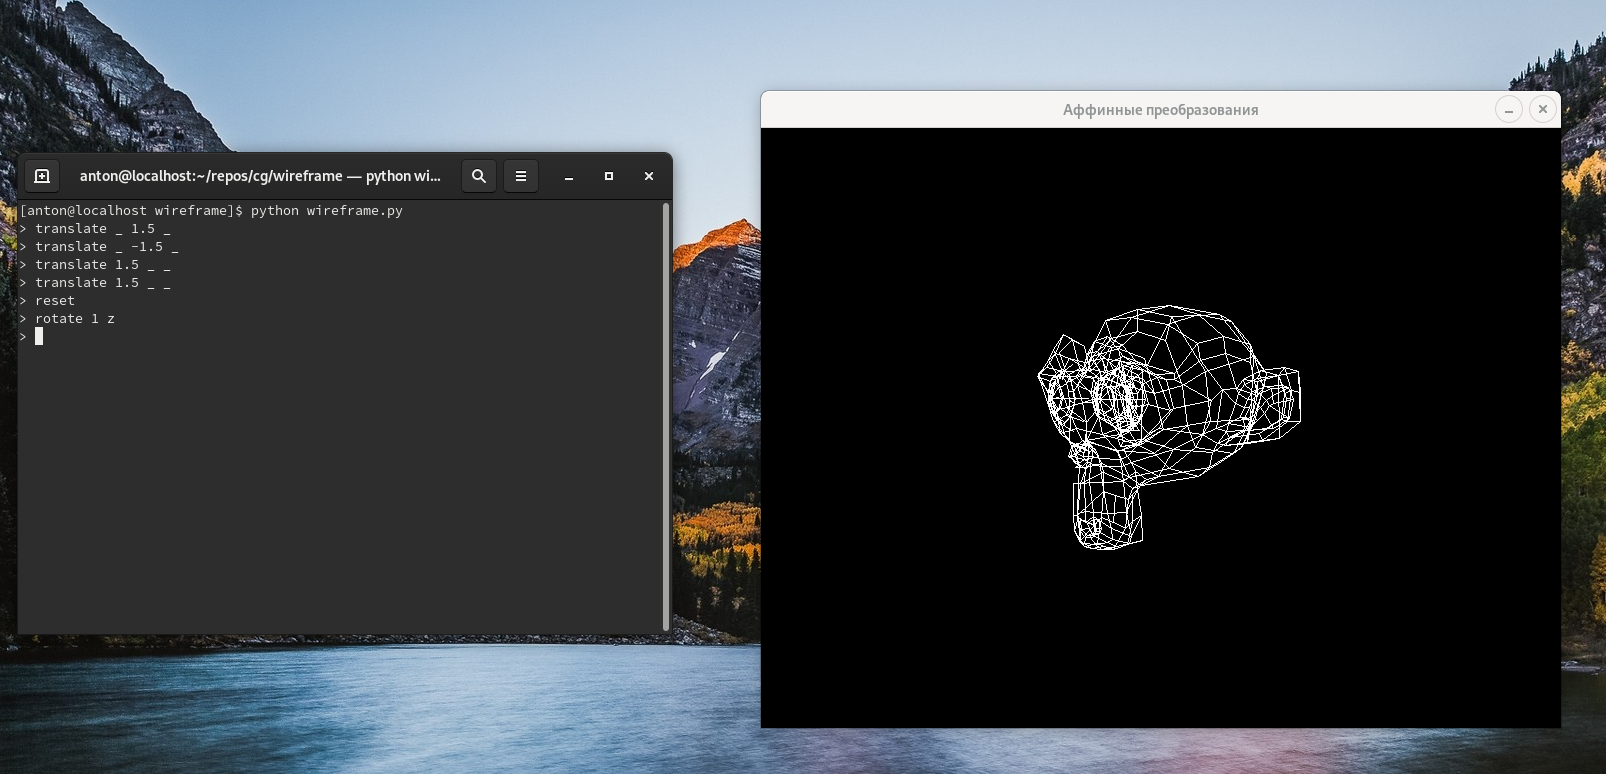
\includegraphics{rotation.png}
  Масштабирование:
  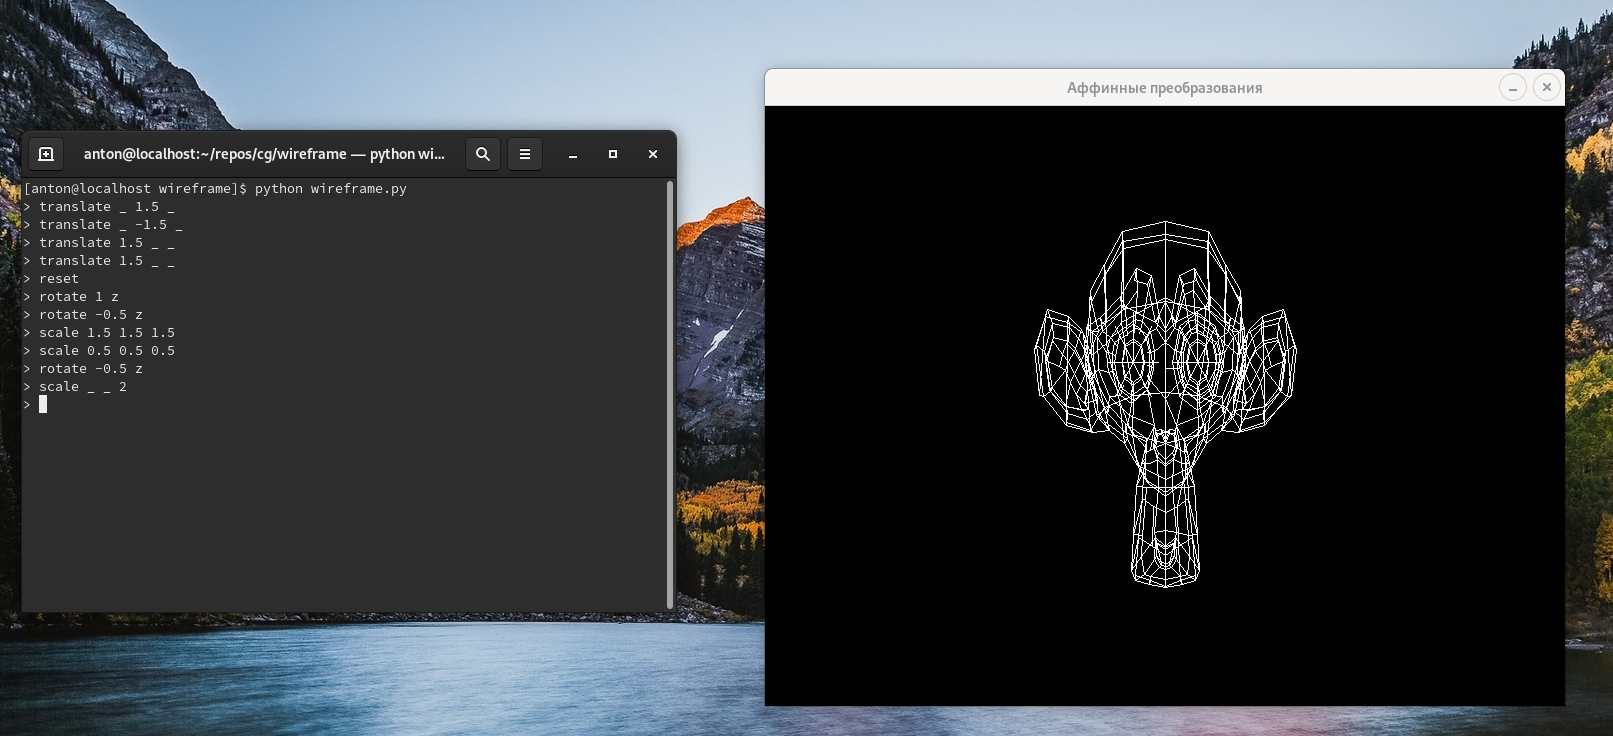
\includegraphics{scale.png}
  Отражение:
  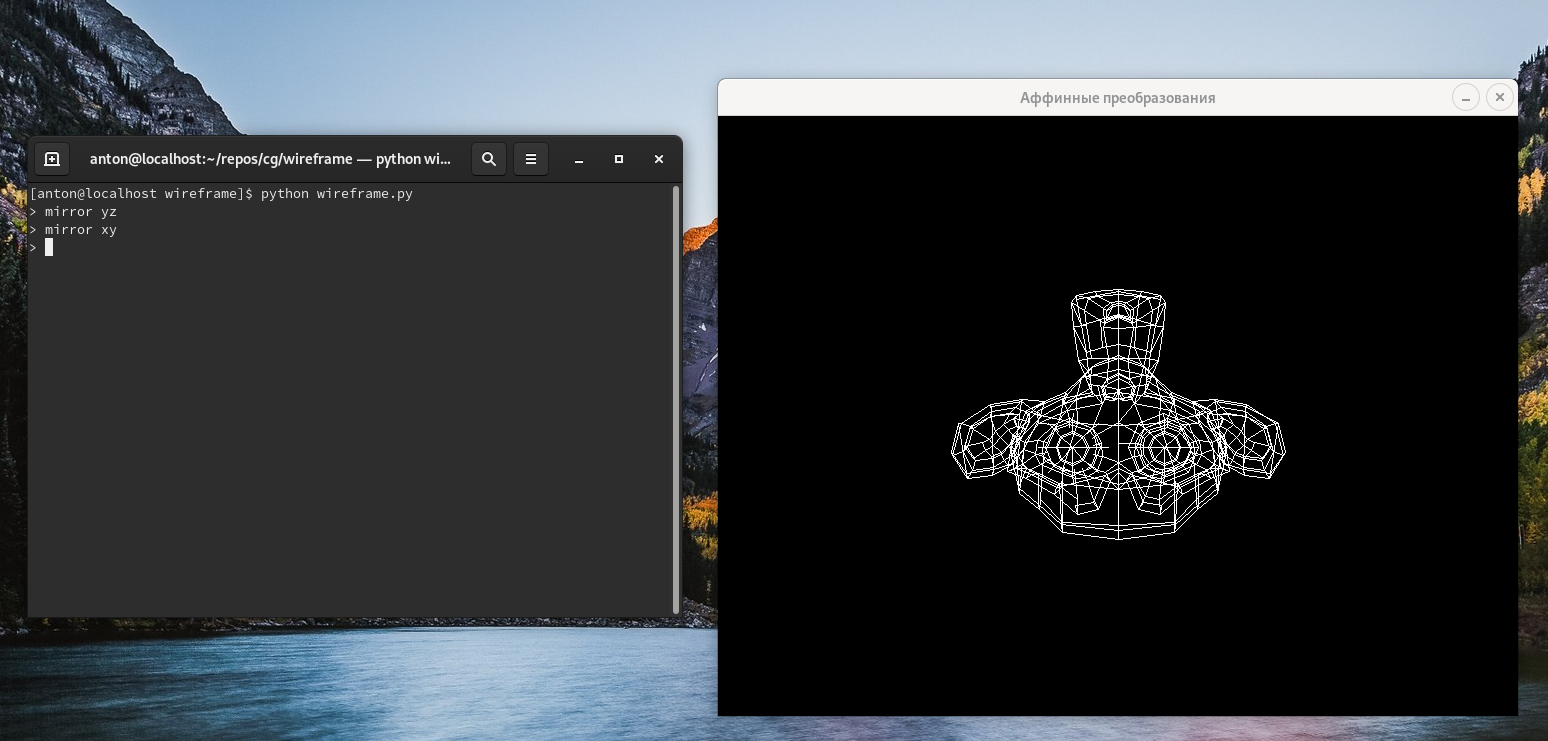
\includegraphics{mirror.png}
  Суперпозиция преобразований:
  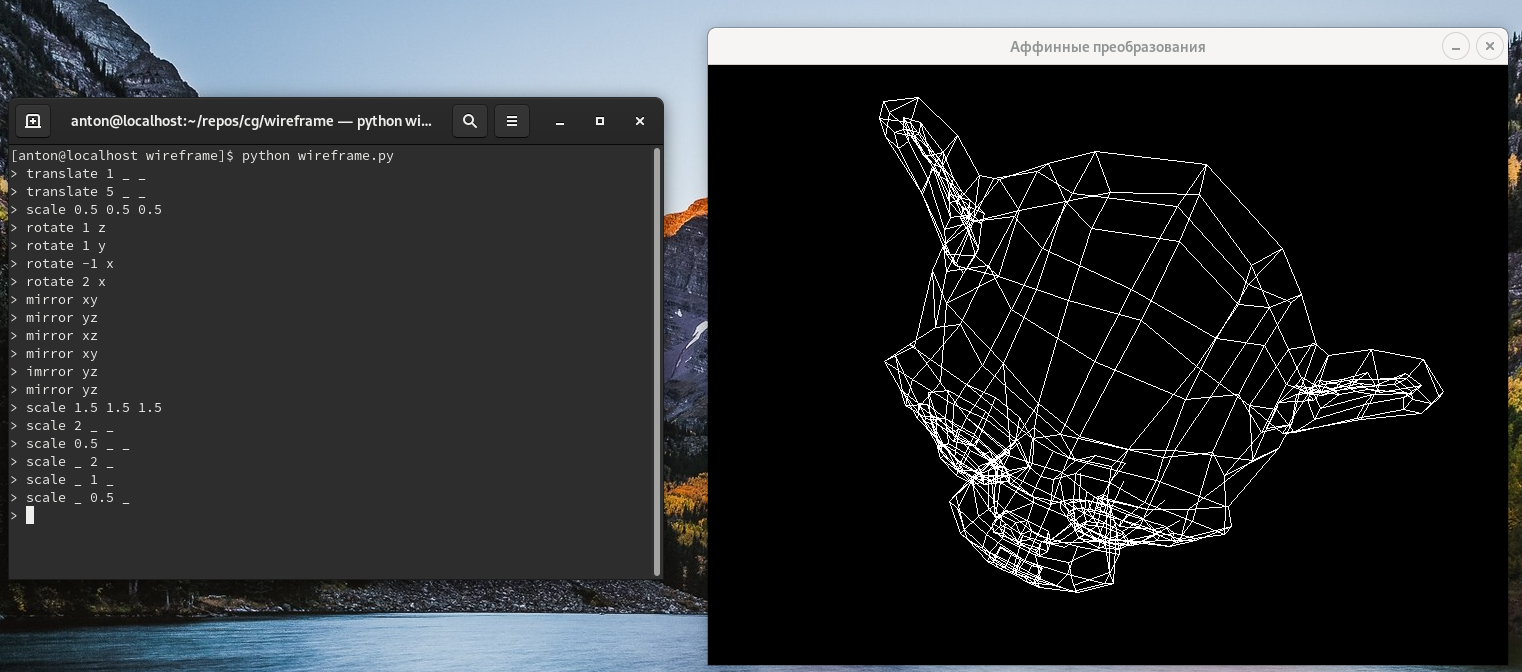
\includegraphics{all_transformations.png}
\end{flushleft}
\begin{flushleft}
  \textbf{Демонстрацию анимации можно посмотреть на YouTube:} \url{https://youtu.be/reCDbkACzpA}
\end{flushleft}
\end{document}

